\subsubsection{Circuitos de activación de los actuadores}

Debido a la alimentación de cada uno de los actuadores propuestos, es necesario realizar circuitos auxiliares para la activación de cada elemento del sistema.

Los motores de aireación, la bomba de agua y la resistencia térmica, requieren de una alimentación de 127 V AC, y el ventilador requiere una alimentación de 12 v DC.

Estos valores no se pueden obtener a la salida de la tarjeta de desarrollo, por lo que es necesario construir un circuito auxiliar, que permita el flujo de la energía requerida después de un estimulo de cambio de estado. 

El circuito seleccionado esta compuesto de un transistor BJT en conexión de emisor común y también se se permitirá el uso de releva dores, para conmutar los estados de encendido y apagado de cada uno de los actuadores, como se observa en la figura \ref{fg:Activacion actuadores}

\begin{figure}[h!]
            \centering
            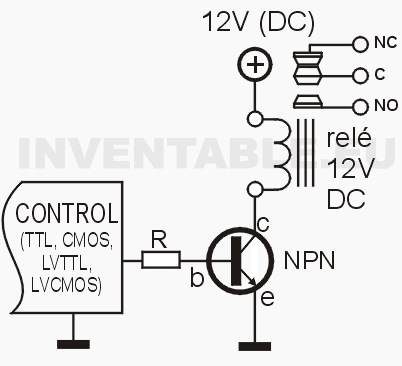
\includegraphics[scale=0.5]{images/Capitulo 4/s5/Rele transistor.png}
            \caption{Circuito de activación de los actuadores \cite{Transis_33}}
            \label{fg:Activacion actuadores}
     \end{figure}

Para adaptar el circuito de la imagen \ref{fg:Activacion actuadores}, se utilizó el transistor 2N2222, con una relevador a 5V DC, y se realizó el calculo para obtener la resistencia de base que amplifique la señal de 3.3 V de la salida de la tarjeta de desarrollo, a los 5 V de la activación del embobinado del relevador.

Para el relevador, en la terminal común, esta la alimentación del actuador, mientras que en el conector normalmente abierto va conectado a tierra y el normalmente cerrado va al actuador. De esta manera, los actuadores se van a activar con una señal lógica alta (1 lógico) .